\subsection{有限维实李群的复化}

引理 7. 设 B 是群，A 是 B 的正规子群，C 是群 B/A，i: A → B 和 p: B → C 是典范态射。设 A' 是群，f 是从 A 到 A' 的同态。设 ω 是从 B 到 A' 的自同构群的态射。假定对于 \(a \in A'\)、\(a' \in A'\)、\(b \in B\)，

\[
f (b a b ^ {- 1}) = \omega (b) f (a), \quad \omega (a) a ^ {\prime} = f (a) a ^ {\prime} f (a) ^ {- 1}.
\]

令 \(\mathbf{B}''\) 为关于 ω 的 \(\mathbf{B}\) 与 \(\mathbf{A}'\)\(\omega\)\(q\) 的半直积，q 为从 \(\mathbf{B}''\) 到 \(\mathbf{B}\) 的典范态射。

\begin{enumerate}
\def\labelenumi{(\roman{enumi})}
\item
  从 A 到 B'' 的映射 \(a \mapsto (f(a^{-1}), i(a))\) 把 A 映到 B'' 的正规子群 D，并且是一个态射。令 B' = B''/D，令 \(i' \colon A' \to B'\)、\(g \colon B \to B'\) 为由 B'' 中 A' 和 B 的典范嵌入取商得到的态射。
\item
  从 \(p \circ q\) 到 \(\mathbf{B}''\) 的态射 \(\mathbf{C}\) 在取商后定义出一个从 \(\mathbf{B}'\) 到 \(\mathbf{C}\) 的态射。
\item
  \(i'\) 是单射，\(p'\) 是满射，\(\operatorname{Ker}(p') = \operatorname{Im}(i')\)，且下图交换
\end{enumerate}

\begin{enumerate}
\def\labelenumi{(\arabic{enumi})}
\setcounter{enumi}{3}
\tightlist
\item
\end{enumerate}

\pandocbounded{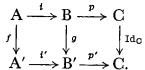
\includegraphics[keepaspectratio]{images/part002_08e8b4be.jpg}}

\begin{enumerate}
\def\labelenumi{(\roman{enumi})}
\setcounter{enumi}{3}
\tightlist
\item
  若 \(b \in \mathbf{B}\) 且 \(a' \in \mathbf{A}'\)，则
\end{enumerate}

\[
g (b) i ^ {\prime} \left(a ^ {\prime}\right) g (b) ^ {- 1} = i ^ {\prime} (\omega (b) a ^ {\prime}).
\]

\begin{enumerate}
\def\labelenumi{(\roman{enumi})}
\tightlist
\item
  对于 A 中的 \(a_{1}\)、\(a_{2}\)，在 B'' 中有
\end{enumerate}

\[
\begin{array}{r l} (f (a _ {1} ^ {- 1}), i (a _ {1})) (f (a _ {2} ^ {- 1}), i (a _ {2})) & = (f (a _ {1} ^ {- 1}) (\omega (a _ {1}) f (a _ {2} ^ {- 1})), i (a _ {1}) i (a _ {2})) \\ & = (f (a _ {1} ^ {- 1}) f (a _ {1} a _ {2} ^ {- 1} a _ {1} ^ {- 1}), i (a _ {1} a _ {2})) \\ & = (f ((a _ {1} a _ {2}) ^ {- 1}, i (a _ {1} a _ {2})) \end{array}
\]

因而 \(a \mapsto (f(a^{-1}), i(a))\)\(h\) 是从 \(A\) 到 \(B''\) 的同态 h。令 \(a \in A\)、\(a' \in A'\)、\(b \in B\)；则在 \(B''\) 中，

\[
\begin{array}{r l} b h (a) b ^ {- 1} & = b f (a ^ {- 1}) a b ^ {- 1} = (\omega (b) f (a ^ {- 1})) (b a b ^ {- 1}) \\ & = f (b a ^ {- 1} b ^ {- 1}) (b a b ^ {- 1}) = h (b a b ^ {- 1}) \\ a ^ {\prime} h (a) a ^ {\prime - 1} & = a ^ {\prime} f (a ^ {- 1}) a a ^ {\prime - 1} = a ^ {\prime} f (a ^ {- 1}) (\omega (a) a ^ {\prime - 1}) a \\ & = a ^ {\prime} f (a ^ {- 1}) f (a) a ^ {\prime - 1} f (a ^ {- 1}) a = h (a) \end{array}
\]

因而 \(h(A) = D\)\(B''\) 是 B'' 的正规子群。

\begin{enumerate}
\def\labelenumi{(\roman{enumi})}
\setcounter{enumi}{1}
\tightlist
\item
  对于 \(a \in A\)，
\end{enumerate}

\[
(p \circ q) (h (a)) = p (q (f (a ^ {- 1}) a)) = p (a) = e
\]

因而 \(p \circ q\) 在 D 上是平凡的。

\begin{enumerate}
\def\labelenumi{(\roman{enumi})}
\setcounter{enumi}{2}
\tightlist
\item
  设 \(a' \in A'\) 满足 \(i'(a') = e\)；则 \(a' \in D\)，因而存在 \(a \in A\) 使得 \(a' = f(a^{-1})a\)；这蕴含 \(a = e\)，从而 \(a' = e\)；故 \(i'\) 是单射。由于 \(p\) 和 \(q\) 是满射，\(p'\) 是满射。
\end{enumerate}

令 \(r\) 表示从 \(B''\) 到 \(B'\) 的典范态射。设 \(a' \in A'\)、\(b \in B\)，且 \(b' = r(a'b)\)。若 \(b' \in \operatorname{Im}(i')\)，则存在 \(a_1' \in A'\) 使得 \(b' = r(a_1')\)；于是存在 \(a \in A\) 使得 \(a'b = a_1'f(a^{-1})a\)，从而 \(b = a \in A\)，且

\[
p ^ {\prime} (b ^ {\prime}) = p (q (a ^ {\prime} b)) = p (b) = e;
\]

因此，\(\operatorname{Im}(i') \subset \operatorname{Ker}(p')\)。仍用 \(a', b, b'\) 表示上述对象，但假设 \(b' \in \operatorname{Ker}(p')\)；于是 \(e = p'(b') = p(q(a'b)) = p(b)\)，从而 \(b \in A\)，故

\[
b ^ {\prime} = r (a ^ {\prime} f (b) f (b ^ {- 1}) b) = r (a ^ {\prime} f (b)) \in \operatorname{Im} (i ^ {\prime});
\]

因此 \(\operatorname{Ker}(p') \subset \operatorname{Im}(i')\)。

若 \(a\in \mathbf{A}\)，则

\[
i ^ {\prime} (f (a)) = r (f (a)) = r (f (a) f \left(a ^ {- 1}\right) a) = r (a) = g (i (a)).
\]

若 \(b\in \mathbf{B}\)，则

\[
p ^ {\prime} (g (b)) = p (b)
\]

从而图 (4) 交换。

\begin{enumerate}
\def\labelenumi{(\roman{enumi})}
\setcounter{enumi}{3}
\tightlist
\item
  设 \(b \in \mathbf{B}\)、\(a' \in \mathbf{A}'\)。则
\end{enumerate}

\[
\begin{array}{r} g (b) i ^ {\prime} (a ^ {\prime}) g (b) ^ {- 1} = r (b) r (a ^ {\prime}) r (b) ^ {- 1} = r (b a ^ {\prime} b ^ {- 1}) \\ = r (\omega (b) a ^ {\prime}) = i ^ {\prime} (\omega (b) a ^ {\prime}). \end{array}
\]

命题 20. 设 G 是有限维实李群。

\begin{enumerate}
\def\labelenumi{(\roman{enumi})}
\item
  存在一个复李群 \(\tilde{\mathbf{G}}\) 和一个从 \(\mathbf{R}\) 到 \(\gamma\) 的 \(\mathbf{G}\)-解析态射 \(\tilde{\mathbf{G}}\)，具有如下性质：对于每个复李群 \(\mathbf{H}\) 以及每个从 \(\mathbf{R}\) 到 \(\phi\) 的 \(\mathbf{G}\)-解析态射 \(\mathbf{H}\)，存在唯一一个从 \(\mathbf{C}\) 到 \(\psi\) 的 \(\tilde{\mathbf{G}}\)-解析态射 \(\mathbf{H}\)，使得 \(\phi = \psi \circ \gamma\)。
\item
  若 \((\tilde{\mathbf{G}}', \gamma')\) 与 \((\tilde{\mathbf{G}}, \gamma)\) 具有相同性质，则存在唯一一个从 \(\theta\) 到 \(\tilde{\mathbf{G}}\) 的同构 \(\tilde{\mathbf{G}}'\)，使得 \(\theta \circ \gamma = \gamma'\)。
\item
  延拓 \(\mathbf{C}\) 的从 \(\mathrm{L}(\mathrm{G}) \otimes \mathbf{C}\) 到 \(\mathrm{L}(\tilde{\mathrm{G}})\) 的 \(\mathrm{L}(\gamma)\)-线性映射是满射；特别地，\(\dim_{\mathbf{C}}(\tilde{\mathbf{G}}) \leqslant \dim_{\mathbf{R}}(\mathrm{G})\)。
\end{enumerate}

断言 (ii) 是显然的。我们证明具有性质 (i) 和 (iii) 的有序对 \((\tilde{G},\gamma)\) 的存在性。

\begin{enumerate}
\def\labelenumi{(\alph{enumi})}
\tightlist
\item
  首先假设 \(G\) 连通。令 \(g = L(G)\)，\(g_{\mathbf{C}} = g \otimes_{\mathbf{R}} \mathbf{C}\) 为 \(g\) 的复化，令 \(S\)（分别地，\(S'\)）为李代数为 \(g\)（分别地，\(g_{\mathbf{C}}\)）的单连通实（分别地，复）李群，并令 \(\sigma\) 为唯一的从 \(\mathbf{R}\) 到 \(S\) 的 \(S'\)-解析态射，使得 \(L(\sigma)\) 是从 \(g\) 到 \(g_{\mathbf{C}}\) 的典范嵌入。令 \(\pi\) 为唯一的从 \(\mathbf{R}\) 到 \(S\) 的 \(G\)-解析态射，使得 \(L(\pi) = I d_{L(G)}\) 且 \(F = K e r \pi\)。
\end{enumerate}

\pandocbounded{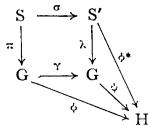
\includegraphics[keepaspectratio]{images/part002_6429af2f.jpg}}

对于每个复李群 H 以及每个从 G 到 H 的 R-解析态射 \(\phi\)，\(L(\phi): g \to L(H)\) 都有唯一的 C-线性延拓到 \(g_{C}\)，且此延拓形如 \(L(\phi^{*})\)，其中 \(\phi^{*}\) 是从 \(S'\) 到 H 的 C-解析态射。于是

\[
\mathrm{L} (\phi \circ \pi) = \mathrm{L} (\phi) \circ \mathrm{L} (\pi) = \mathrm{L} (\phi) = \mathrm{L} (\phi^ {*}) \circ \mathrm{L} (\sigma) = \mathrm{L} (\phi^ {*} \circ \sigma)
\]

因而 \(\phi \circ \pi = \phi^{*} \circ \sigma\)。所以 \(\phi^{*}(\sigma(F)) = \phi(\pi(F)) = \{e\}\)，从而

\[
\sigma (\mathrm{F}) \subset \operatorname{Ker} \phi^ {*}.
\]

令 P 为所有 \(\phi^{*}\) 变化时的 Ker \(\phi\) 的交。这是 \(S'\) 的正规李子群（第 2 号，命题 1 的推论 3）。令 \(\tilde{G} = S'/P\)，令 \(\lambda: \mathbf{S}' \to \tilde{\mathbf{G}}\) 为典范态射。于是 \(\sigma(\mathbf{F}) \subset \mathbf{P}\)，因而存在唯一一个从 \(\mathbf{R}\) 到 \(\gamma\) 的 \(\mathbf{G}\)-解析态射 \(\tilde{\mathbf{G}}\)，使得 \(\gamma \circ \pi = \lambda \circ \sigma\)。若 \(\psi: \tilde{\mathbf{G}} \to \mathbf{H}\) 表示由 \(\phi^*\) 在取商时导出的态射，则

\[
(\phi \circ \gamma) \circ \pi = \psi \circ (\lambda \circ \sigma) = \phi^ {*} \circ \sigma = \phi \circ \pi
\]

从而 \(\psi \circ \gamma = \phi\)。显然，\(\mathrm{L}(\psi)\)，进而 \(\psi\)，由等式 \(\psi \circ \gamma = \phi\) 唯一确定。因此我们证明了有序对 \((\tilde{G}, \gamma)\) 具有性质 (i) 和 (iii)。

\begin{enumerate}
\def\labelenumi{(\alph{enumi})}
\setcounter{enumi}{1}
\tightlist
\item
  现在转到一般情形。令 \(\mathbf{F}\) 为 \(\mathrm{G},\mathrm{M} = \mathrm{G} / \mathrm{F}\) 的单位分支，，令 \(i\colon \mathrm{F}\to \mathrm{G}\) 和 \(p\colon \mathrm{G}\rightarrow \mathrm{M}\) 为典范态射。我们将证明的部分 (a) 应用于 F。得到有序对 \((\tilde{\mathbf{F}},\delta)\)。对于所有 \(g\in \mathrm{G}\)，内自同构 Int \(g|\mathrm{F} = \omega '(g)\) 是 F 的自同构。由 \(\tilde{\mathbf{F}}\) 的泛性质，存在唯一一个复李群 \(\omega (g)\) 的自同构 \(\tilde{\mathbf{F}}\)，使得 \(\delta \circ \omega '(g) = \omega (g)\circ \delta\)。显然，\(\omega\) 是从 G 到 \(\operatorname {Aut}(\tilde{\mathbf{F}})\) 的态射。若 \(g\in \mathbf{G}\) 且 \(f\in \tilde{\mathbf{F}}\)，则
\end{enumerate}

\[
\delta (g f g ^ {- 1}) = (\delta \circ \omega^ {\prime} (g)) (f) = (\omega (g) \circ \delta) (f) = \omega (g) (\delta (f)).
\]

若 \(f \in \mathbf{F}\)，则 \(\delta \circ (\operatorname{Int}_{\mathbb{F}} f) = (\operatorname{Int}_{\tilde{\mathbb{F}}} \delta(f)) \circ \delta\)，且 \(\operatorname{Int}_{\tilde{\mathbb{F}}} \delta(f)\) 是复李群 \(\tilde{\mathbf{F}}\) 的自同构；故 \(\operatorname{Int}_{\tilde{\mathbb{F}}} \delta(f) = \omega(f)\)。

因此可应用引理 7，从而得到交换图

\[
\begin{array}{c} \mathrm{F} \xrightarrow {i} \mathrm{G} \xrightarrow {p} \mathrm{M} \\ \delta \Big \downarrow \qquad \qquad \qquad \gamma \Big \downarrow \qquad \qquad \Big \downarrow \mathrm{Id} \\ \tilde {\mathrm{F}} \xrightarrow {\tilde {i}} \tilde {\mathrm{G}} \xrightarrow {\tilde {p}} \mathrm{M}. \end{array}
\]

借助 \(\tilde{\mathbf{F}}\)，将 \(\tilde{\mathbf{G}}\) 识别为 \(\tilde{i}\) 的正规子群。群 \(\tilde{\mathbf{G}}\) 由 \(\tilde{\mathbf{F}}\) 和 \(\gamma (\mathbf{G})\) 生成；因此，由 \(\tilde{\mathbf{F}}\) 的元素定义的 \(\tilde{\mathbf{G}}\) 的自同构都是复李群结构的自同构。由 § 1，第 9 号，命题 18，\(\tilde{\mathbf{G}}\) 上存在唯一一个复李群结构，使得 \(\tilde{\mathbf{F}}\) 是 \(\tilde{\mathbf{G}}\) 的开李子群。以下 \(\tilde{\mathbf{G}}\) 均取此结构。由于 \(\delta\) 是 \(\mathbf{R}\)-解析的，\(\gamma\) 也是 \(\mathbf{R}\)-解析的。

有序对 \((\tilde{G},\gamma)\) 具有命题的性质 (iii)。我们证明它具有性质 (i)。设 H 是复李群，\(\phi\) 是从 G 到 H 的 R-解析态射。存在一个从 \(\eta\) 到 H 的 C-解析态射 \(\tilde{F}\)，使得 \(\eta \circ \delta = \phi |F\)。设 \(g\in G\)。映射

\[
f \mapsto \eta (\omega (g) f), \quad f \mapsto \phi (g) \eta (f) \phi (g) ^ {- 1}
\]

从 \(\tilde{\mathbf{F}}\) 到 \(\mathbf{H}\) 都是 \(\mathbf{C}\)-解析态射；它们在 \(\delta(\mathbf{F})\) 上一致，因为若 \(f' \in \mathbf{F}\)，则

\[
\begin{array}{r} \phi (g) \eta (\delta (f ^ {\prime})) \phi (g) ^ {- 1} = \phi (g) \phi (f ^ {\prime}) \phi (g) ^ {- 1} = \phi (g f ^ {\prime} g ^ {- 1}) \\ = \eta (\delta (g f ^ {\prime} g ^ {- 1})) = \eta (\omega (g) \delta (f ^ {\prime})); \end{array}
\]

因此对于所有 \(\eta (\omega (g)f) = \phi (g)\eta (f)\phi (g)^{-1}\) 和所有 \(g\in G\)，都有 \(f\in \tilde{\mathbf{F}}\)。若 \(\mathbf{G}'\) 表示关于 \(\mathbf{G}\) 的 \(\tilde{\mathbf{F}}\) 与 \(\omega\) 的半直积，则存在从群 \(\zeta\) 到 \(\mathbf{G}'\) 的态射 \(\mathrm{H}\)，它在 \(\phi\) 上与 \(\mathrm{G}\) 一致，在 \(\eta\) 上与 \(\tilde{\mathbf{F}}\) 一致。对于 \(f\in \mathbf{F}\)，

\[
\zeta (\delta (f ^ {- 1}) f) = \eta (\delta (f ^ {- 1})) \phi (f) = \phi (f ^ {- 1}) \phi (f) = e.
\]

因此 \(\zeta\) 在取商后定义出从 \(\psi\) 到 H 的态射 \(\tilde{\mathbf{G}}\)。于是 \(\psi \circ \gamma = \phi\) 且 \(\psi \circ \tilde{i} = \eta\)；后一个等式蕴含 \(\psi\) 是 C-解析的。

最后，设 \(\psi'\) 是从 \(\mathbf{C}\) 到 \(\tilde{\mathbf{G}}\) 的 \(\mathbf{H}\)-解析态射，满足 \(\phi = \psi' \circ \gamma\)。则

\[
\psi^ {\prime} \circ \tilde {i} \circ \delta = \psi^ {\prime} \circ \gamma \circ i = \phi \circ i = \psi \circ \tilde {i} \circ \delta
\]

因而 \(\psi' \circ \tilde{i} = \psi \circ \tilde{i}\)。由于 \(\tilde{G}\) 由 \(\tilde{i}(\tilde{\mathrm{F}})\) 和 \(\gamma(G)\) 生成，\(\psi' = \psi\)。

定义 4. \((\tilde{G},\gamma)\)，或简记为 \(\tilde{G}\)，称为 G 的泛复化。

注记。(1) 设 \((\tilde{\mathbf{G}},\gamma)\) 是 G 的泛复化。设 \(G_0\)（分别地，\(\tilde{G}_0\)）为 G（分别地，\(\tilde{G}\)）的单位分支。由命题 20 的证明，\((\tilde{G}_0,\gamma |G_0)\) 是 \(G_0\) 的泛复化，且复合态射

\[
\mathrm{G} \rightarrow \tilde {\mathrm{G}} \rightarrow \tilde {\mathrm{G}} / \tilde {\mathrm{G}} _ {0}
\]

在取商后定义出从 \(\mathbf{G} / \mathbf{G}_0\) 到 \(\tilde{\mathbf{G}} / \tilde{\mathbf{G}}_0\) 的同构。

\begin{enumerate}
\def\labelenumi{(\arabic{enumi})}
\setcounter{enumi}{1}
\tightlist
\item
  假设 G 单连通。令 \(g = L(G)\)，令 \(g_{c}\) 为 g 的复化，令 \(S'\) 为李代数为 \(g_{c}\) 的单连通复李群，令 \(\sigma\) 为从 G 到 \(S'\) 的态射，使得 \(L(\sigma)\) 是从 g 到 \(g_{c}\) 的典范嵌入。我们再次使用命题 20 的证明中部分 (a) 的记号。若 \(H = S'\) 且 \(\phi = \sigma\)，则 \(\phi^{*} = I d_{g}\)。因此 \((S', \sigma)\) 是 G 的泛复化。注意 \(\sigma\) 一般并非单射（练习 16）；然而由于 \(L(\sigma)\) 是单射，其核是离散的。另一方面，令 \(\theta\) 为由 g 定义的 \(g_{c}\) 的对合，令 \(\eta\)\(S'\) 为 S' 的底层实李群所对应的自同构；令 \(S'^{\eta}\)\(S'\) 为 S' 中在 \(\eta\)\(S'\) 下不变的点的集合；它是 S' 的实李子群，其李代数为 g（§3，第 8 号，命题 29 的推论 1）。由第 1 号、命题 1 的推论 1，\(\sigma(G)\)\(S'\) 是 S' 的李代数为 g 的实积分子群，因而 \(\sigma(G)\) 是 \(S'^{\eta}\) 的单位分支；特别地，\(\sigma(G)\)\(S'\) 是 S' 的实李子群。
\end{enumerate}

